\section{Physics of Basic Semiconductor Devices}
\title[Physics]{Physics of basic semiconductor devices}  

\begin{frame}[plain]
    \titlepage
\end{frame}

%%%%%%%%%%%%%%%%%%%%%%%%%%%%%%%%%%%%%%%%%%%%%%%%%%%%%%%%%%%%%
%% Introduction to the module %%
%%%%%%%%%%%%%%%%%%%%%%%%%%%%%%%%%%%%%%%%%%%%%%%%%%%%%%%%%%%%%
\begin{frame}
    \frametitle{What will you learn?}
\begin{itemize}
    \item Materials
        \begin{itemize}
            \item Atoms and materials used in semiconductors
            \item Flow of electrons and holes
            \item Conductors, insulators, and semiconductors
            \item Energy bands, Fermi level, doping
            \item Intrinsic and extrinsic semiconductors
        \end{itemize}
    \item Fundamental properties
        \begin{itemize}
            \item Carrier concentration 
            \item Carrier mobility
            \item The Hall effect
            \item Drift and diffusion currents
            \item Breakdown voltage, temerature dependence, etc.
        \end{itemize}
    \item pn junctions
        \begin{itemize}
            \item What is a pn junction?
            \item Diodes and their characteristics
            \item Physics of operaiton, properties and IV characteristics of diodes.
        \end{itemize}
\end{itemize}
\end{frame}

%%%%%%%%%%%%%%%%%%%%%%%%%%%%%%%%%%%%%%%%%%%%%%%%%%%%%%%%%%%%%
%% Atoms %%
%%%%%%%%%%%%%%%%%%%%%%%%%%%%%%%%%%%%%%%%%%%%%%%%%%%%%%%%%%%%%
\begin{frame}
	\frametitle{Atoms}
	\begin{columns}
		\begin{column}{0.65\textwidth}
          \begin{itemize}
            \item All matter is made up of atoms.
            \item Atoms are the smallest unit of matter that retains the properties of an element.
            \item Two models of atom exist: classical and quantum.
            \item The classical model of the atom is based on the idea that atoms are made up of a nucleus (protons and neutrons) surrounded by electrons that orbit the nucleus in fixed paths- Rutherford's Atomic Model
            \item The quantum model of the atom is based on the principles of quantum mechanics, which describe the behaviour of particles at the atomic and subatomic quantised energy levels- Bohr's Atomic Model:
            \item Both model states: atoms consist of a nucleus (protons \& neutrons) \& electrons that orbit the nucleus.
          \end{itemize}
		\end{column}
        \hfill
		\begin{column}{0.35\textwidth}
            \begin{figure}
                \centering
                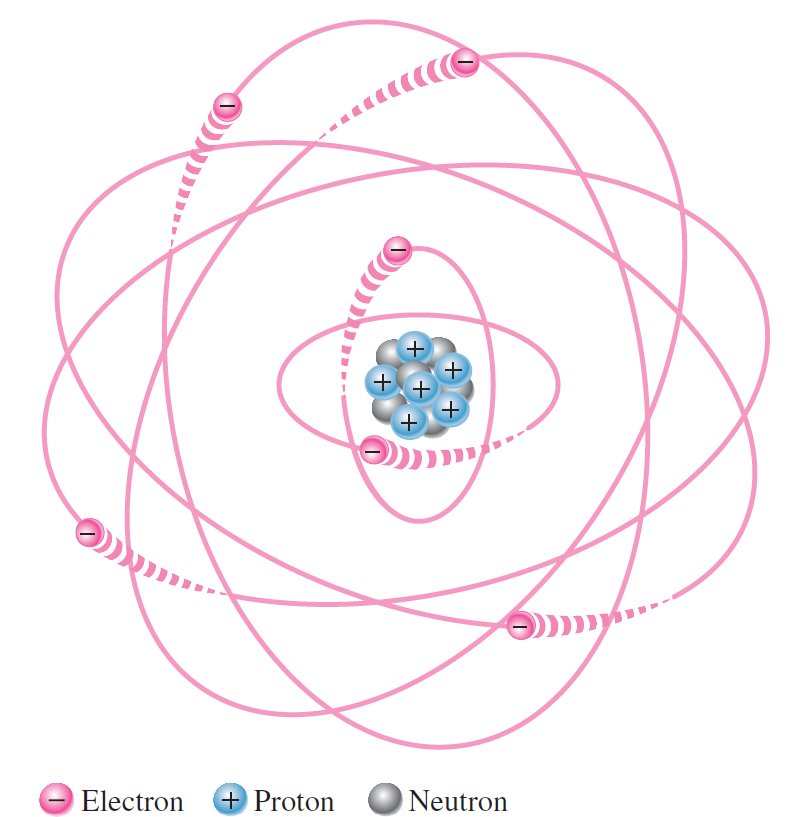
\includegraphics[width=0.8\textwidth]{fig/lec02/Atom_model.png}
                \caption{The Bohr model of an atom (Adapted from \href{https://www.pearson.com/en-us/subject-catalog/p/electronic-devices-electron-flow-version/P200000001048/9780137556755}{Electronic Devices (Electron Flow Version), 10th edition})}
            \end{figure}
		\end{column}
		\end{columns}
\end{frame}


%%%%%%%%%%%%%%%%%%%%%%%%%%%%%%%%%%%%%%%%%%%%%%%%%%%%%%%%%%%%%
%% Atoms continued %%
%%%%%%%%%%%%%%%%%%%%%%%%%%%%%%%%%%%%%%%%%%%%%%%%%%%%%%%%%%%%%
\begin{frame}
	\frametitle{Atoms}
	\begin{columns}
		\begin{column}{0.65\textwidth}
          \begin{itemize}
            \item The number of protons in the nucleus determines the element (e.g., hydrogen, oxygen, etc.).
            \item Electrons are arranged in energy levels or shells around the nucleus.
            \item Electrons are negatively charged, while protons are positively charged.
            \item Number of protons in the nucleus is equal to the number of electrons in the atom, making it electrically neutral.
            \item Outermost shell of an atom is called the valence shell.
            \item Number of electrons in the valence shell, also called valence electrons determines the chemical properties of the atom.
            \item Atoms can gain or lose electrons to form ions, which are charged particles.
          \end{itemize}
		\end{column}
        \hfill
		\begin{column}{0.35\textwidth}
            \begin{figure}
                \centering
                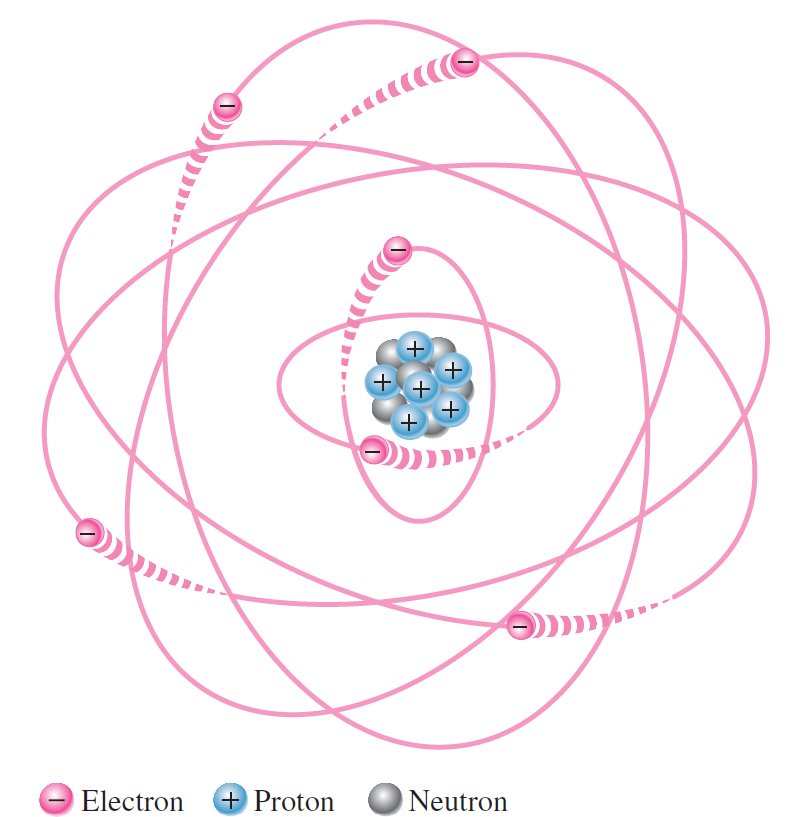
\includegraphics[width=0.8\textwidth]{fig/lec02/Atom_model.png}
                \caption{The Bohr model of an atom (Adapted from \href{https://www.pearson.com/en-us/subject-catalog/p/electronic-devices-electron-flow-version/P200000001048/9780137556755}{Electronic Devices (Electron Flow Version), 10th edition})}
            \end{figure}
		\end{column}
		\end{columns}
\end{frame}

%%%%%%%%%%%%%%%%%%%%%%%%%%%%%%%%%%%%%%%%%%%%%%%%%%%%%%%%%%%%%
%% Ionisation energy %%
%%%%%%%%%%%%%%%%%%%%%%%%%%%%%%%%%%%%%%%%%%%%%%%%%%%%%%%%%%%%%
\begin{frame}
	\frametitle{Ionisation energy}
          \begin{itemize}
            \item The energy required to remove an electron from an atom is called ionisation energy.
            \item The ionisation energy varies for different elements and is generally higher for elements with more protons in the nucleus.
            \item The ionisation energy is also affected by the distance of the electron from the nucleus and the number of electrons in the valence shell- outermost shell is more vulnerable to ionisation!
            \item Atoms with low ionisation energy tend to lose electrons easily and form positive ions, while atoms with high ionisation energy tend to gain electrons and form negative ions.
            \item The ionisation energy is an important factor in determining the chemical reactivity of an element.
          \end{itemize}
\end{frame}


%%%%%%%%%%%%%%%%%%%%%%%%%%%%%%%%%%%%%%%%%%%%%%%%%%%%%%%%%%%%%
%% Materials %%
%%%%%%%%%%%%%%%%%%%%%%%%%%%%%%%%%%%%%%%%%%%%%%%%%%%%%%%%%%%%%
\begin{frame}
	\frametitle{Materials in electronics}
	\begin{columns}
		\begin{column}{0.6\textwidth}
            \begin{itemize}
                \item The electrical properties of materials are determined by the arrangement and behaviour of their atoms and electrons.
                \item Example: Carbon (C) has 4 valence electrons.
                \item Nucleus of C: has 6 protons and 6 neutrons. 2 electrons in the inner shell/core make a charge of +4 in the core.
                \item 4 valence electrons in the outer shell, forms covalent bonds with other atoms. 
                \item In solids like diamond or any organic compounds, each carbon atom is tightly bonded to 4 others in a 3D lattice — \textbf{no free electrons to move around}.
                \item So, carbon is a non-metal and is a poor conductor of electricity. 
            \end{itemize}
		\end{column}
        \hfill
		\begin{column}{0.4\textwidth}
            \begin{figure}
                \centering
                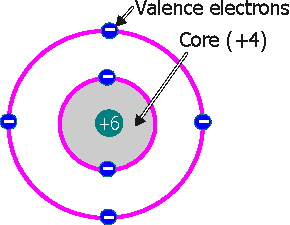
\includegraphics[width=0.8\textwidth]{fig/lec02/carbon_atom.pdf}
                \caption{Carbon atom with four valence electrons- used in resistors but if you \textbf{change crystal structure} (example graphite, where one electron is free to move due to flat layers of carbon atoms)}
            \end{figure}
		\end{column}
		\end{columns}
\end{frame}

%%%%%%%%%%%%%%%%%%%%%%%%%%%%%%%%%%%%%%%%%%%%%%%%%%%%%%%%%%%%%
%% Insulators, conductors and semiconductors %%
%%%%%%%%%%%%%%%%%%%%%%%%%%%%%%%%%%%%%%%%%%%%%%%%%%%%%%%%%%%%%
\begin{frame}
	\frametitle{Materials in electronics}
            \begin{itemize}
                \item The electrical properties of materials can be classified into three categories based on their ability to conduct electricity:
            \begin{itemize}
                \item \textbf{Insulators} have valence electrons tightly bound to the atoms and do not have free electrons to conduct electricity. Insulators have a \textbf{very high ionisation energy}, meaning they require a lot of energy to remove an electron from the atom. So they are bad conductors of electricity. Examples: rubber, glass, and plastic.
                \item \textbf{Conductors} have a large number of loosly bounded electrons that can move easily through the material, allowing them to conduct electricity well. Conductors have a \textbf{low ionisation energy}, meaning they require very little energy to remove an electron from the atom. So, they have a low resistance to the flow of electric current. Examples: metals like copper (Cu) and aluminum (Al).
                \item \textbf{Semiconductors*} in pure or intrinsic state is neither a good conductor nor a good insulator. They have to be synthesized as compounds or made extrinsic by adding impurities (doping) to change their electrical properties. Examples: Silicon (Si) and Germanium (Ge) as intrinsic and gallium arsenide, indium phosphide, gallium nitride, silicon carbide are extrinsic.
            \end{itemize}
            \end{itemize}
            *Semiconductors can conduct electricity under certain conditions, such as when they are doped with impurities or when they are exposed to light or heat.
\end{frame}

%%%%%%%%%%%%%%%%%%%%%%%%%%%%%%%%%%%%%%%%%%%%%%%%%%%%%%%%%%%%%
%% Ask about explanation based on Bohr model of atom %%
%%%%%%%%%%%%%%%%%%%%%%%%%%%%%%%%%%%%%%%%%%%%%%%%%%%%%%%%%%%%%
\begin{frame}
	\frametitle{Example explanation based on Bohr model of atom}
        \begin{figure}
            \centering
            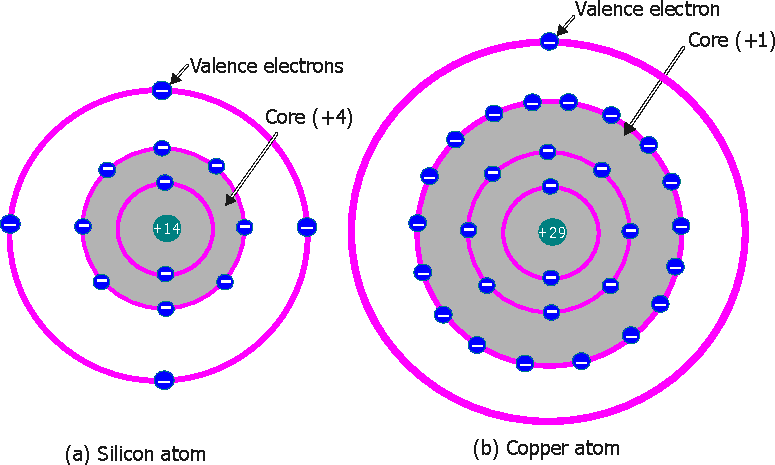
\includegraphics[width=0.7\textwidth]{fig/lec02/Cu_Si_atom1.pdf}
            \caption{(a) Silicon atom with four valence electrons, (b) Copper atom with one valence electron}
        \end{figure}
\end{frame}

%%%%%%%%%%%%%%%%%%%%%%%%%%%%%%%%%%%%%%%%%%%%%%%%%%%%%%%%%%%%%
%% Explanation based on Bohr model of atom %%
%%%%%%%%%%%%%%%%%%%%%%%%%%%%%%%%%%%%%%%%%%%%%%%%%%%%%%%%%%%%%
\begin{frame}
	\frametitle{Example explanation based on Bohr model of atom}
	\begin{columns}
		\begin{column}{0.6\textwidth}
            \begin{itemize}
                \item \textbf{Semiconductor}: Silicon
                \item Silicon (Si) has 4 valence electrons.
                \item Nucleus of Si: has 14 protons and 14 neutrons. 10 electrons in the inner shell/core make a charge of +4 in the core.
                \item 4 valence electrons in the outer shell, forms covalent bonds with other atoms.
                \item In solids like those forming an organic compounds, each silicon atom is tightly bonded to 4 others in a 3D lattice — \textbf{no free electrons to move around}.
                \item So, silicon is a non-metal and is a poor conductor of electricity.
            \end{itemize}
		\end{column}
        \hfill
		\begin{column}{0.4\textwidth}
            \begin{figure}
                \centering
                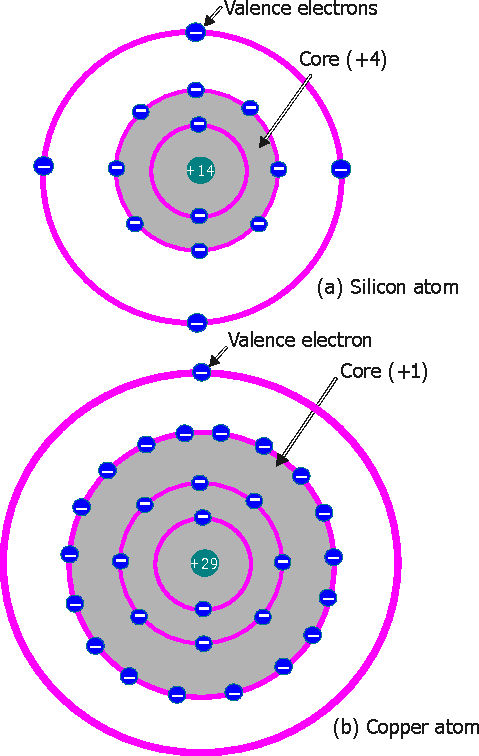
\includegraphics[width=0.6\textwidth]{fig/lec02/Cu_Si_atom.pdf}
                \caption{(a) Silicon atom with four valence electrons, (b) Copper atom with one valence electron}
            \end{figure}
		\end{column}
		\end{columns}
\end{frame}

%%%%%%%%%%%%%%%%%%%%%%%%%%%%%%%%%%%%%%%%%%%%%%%%%%%%%%%%%%%%%
%% Explanation based on Bohr model of atom %%
%%%%%%%%%%%%%%%%%%%%%%%%%%%%%%%%%%%%%%%%%%%%%%%%%%%%%%%%%%%%%
\begin{frame}
	\frametitle{Example explanation based on Bohr model of atom}
	\begin{columns}
		\begin{column}{0.6\textwidth}
            \begin{itemize}
                \item \textbf{Conductor}: Copper
                \item Copper (Cu) has 1 valence electron.  
                \item Nucleus of Cu: has 29 protons and 29 neutrons. 28 electrons in the inner shell/core make a charge of +1 in the core.
                \item 1 valence electron in the outer shell, forms metallic bonds with other atoms.
                \item In solids like copper, each copper atom is loosely bonded to other atoms in a 3D lattice — \textbf{free electrons to move around}.
                \item So, copper is a metal and is a good conductor of electricity.
            \end{itemize}
		\end{column}
        \hfill
		\begin{column}{0.4\textwidth}
            \begin{figure}
                \centering
                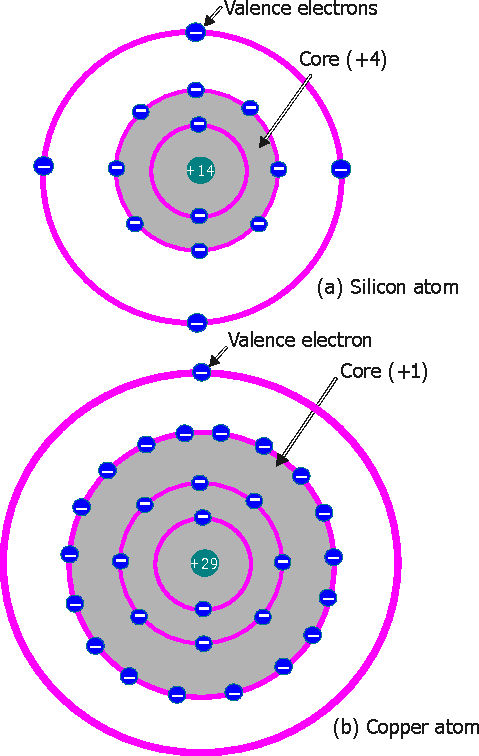
\includegraphics[width=0.6\textwidth]{fig/lec02/Cu_Si_atom.pdf}
                \caption{(a) Silicon atom with four valence electrons, (b) Copper atom with one valence electron}
            \end{figure}
		\end{column}
		\end{columns}
\end{frame}

%%%%%%%%%%%%%%%%%%%%%%%%%%%%%%%%%%%%%%%%%%%%%%%%%%%%%%%%%%%%%
%% Total energy of the electron %%
%%%%%%%%%%%%%%%%%%%%%%%%%%%%%%%%%%%%%%%%%%%%%%%%%%%%%%%%%%%%%
\begin{frame}
	\frametitle{Energy of electron in an orbit}
    \begin{columns}
        \begin{column}{0.6\textwidth}
            \begin{itemize}
                \item The energy of an electron in an orbit is determined by the distance of the electron from the nucleus and the number of protons in the nucleus.
                \item Electrons in orbits closer to the nucleus have lower energy than those in orbits farther away.
                \item The energy of an electron in an orbit is also affected by the presence of other electrons in the atom.
                \item Electrons in the same shell repel each other, which can increase their energy and make them more likely to be ionised.
                \item \textbf{Why is electron having a negative charge?}
            \end{itemize}
        \end{column}
        \hfill
        \begin{column}{0.4\textwidth}
            \begin{figure}
                \centering
                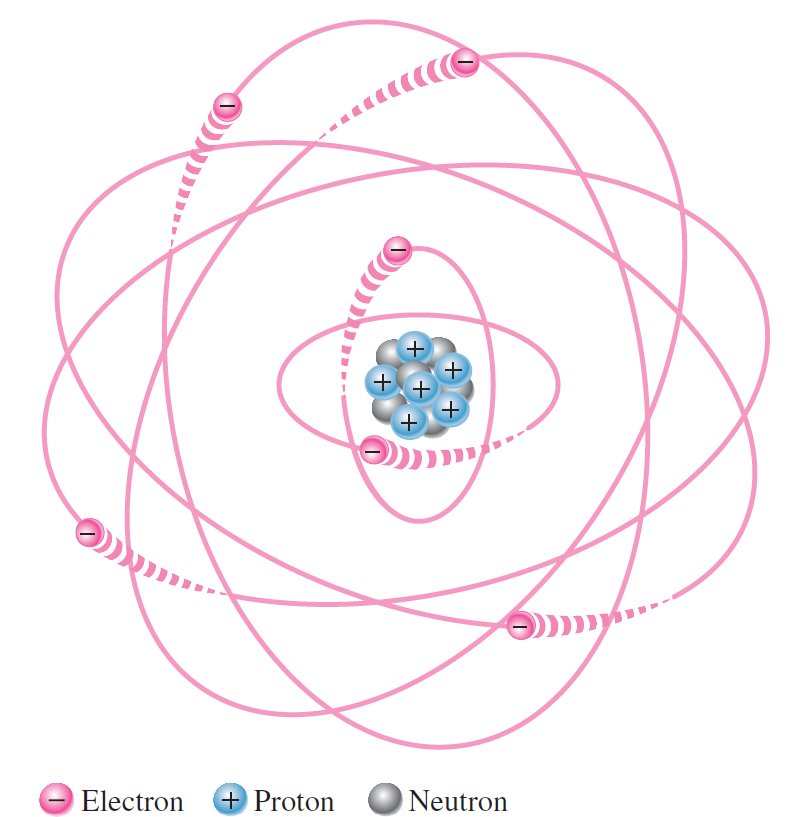
\includegraphics[width=0.8\textwidth]{fig/lec02/Atom_model.png}
                \caption{The Bohr model of an atom (Adapted from \href{https://www.pearson.com/en-us/subject-catalog/p/electronic-devices-electron-flow-version/P200000001048/9780137556755}{Electronic Devices (Electron Flow Version), 10th edition})}
            \end{figure}
        \end{column}
        \end{columns}
\end{frame}

%%%%%%%%%%%%%%%%%%%%%%%%%%%%%%%%%%%%%%%%%%%%%%%%%%%%%%%%%%%%%
%% Total energy of the electron %%
%%%%%%%%%%%%%%%%%%%%%%%%%%%%%%%%%%%%%%%%%%%%%%%%%%%%%%%%%%%%%
\begin{frame}
	\frametitle{Total energy of the electron}
    \begin{itemize}
        \item The planetary model of atom developed by \textbf{Niels Bohr} in 1913, where electrons are thought to orbit the nucleus like planets orbiting the sun. \textit{The nucleus is considered fixed in space.}
        \item We aim to derive the total energy $W$ of the electron.
        \item Electrostatic force of attraction between the electron and the nucleus (Coulomb's law):
        \begin{equation}
            \frac{q^2}{4 \pi \varepsilon_0 r^2}
        \end{equation}  where $q$ is the charge of the electron, $\varepsilon_0$ is the permittivity of free space, and $r$ is the distance between the electron and the nucleus.
        \item Centripetal force of electron in circular motion assuming mass $m$ and $v$ is its velocity:
        \begin{equation}
            \frac{mv^2}{r}
        \end{equation}
        \item Equating forces (from Newton's second law of motion):
        \begin{equation} \label{eq:Newton}
            \frac{q^2}{4 \pi \varepsilon_0 r^2} = \frac{mv^2}{r}
        \end{equation}
    \end{itemize}
\end{frame}

%%%%%%%%%%%%%%%%%%%%%%%%%%%%%%%%%%%%%%%%%%%%%%%%%%%%%%%%%%%%%
%% Explanation why electro is negative %%
%%%%%%%%%%%%%%%%%%%%%%%%%%%%%%%%%%%%%%%%%%%%%%%%%%%%%%%%%%%%%
\begin{frame}
	\frametitle{Total energy of the electron}
    \begin{columns}
        \begin{column}{0.5\textwidth}
            \begin{itemize}
                \item Potential energy of the electron at a distance r from the nucleus:
                \begin{equation}
                U = -\frac{q^2}{4 \pi \varepsilon_0 r}
                \end{equation}
                
                \item Kinetic energy:
                \begin{equation}
                K = \frac{1}{2}mv^2
                \end{equation}
                
                \item Total Energy:
                \begin{equation} \label{eq:total_energy}
                W = K + U = \frac{1}{2}mv^2 - \frac{q^2}{4 \pi \varepsilon_0 r}
                \end{equation}
                
            \end{itemize}
        \end{column}
        
        \hfill
        
        \begin{column}{0.5\textwidth}
            \centering
            \begin{itemize}
                \item From \ref{eq:Newton} we can substitute for $mv^2$:
                \begin{equation}
                mv^2 = \frac{q^2}{4 \pi \varepsilon_0 r}
                \end{equation}

                \item Substituting in \ref{eq:total_energy} gives:
                \begin{equation}
                W = \frac{1}{2} \cdot \frac{q^2}{4 \pi \varepsilon_0 r} - \frac{q^2}{4 \pi \varepsilon_0 r}
                \end{equation}
                
                \item Simplifies to:
                \begin{equation}
                W = -\frac{q^2}{8 \pi \varepsilon_0 r}
                \end{equation}
            \end{itemize}
        \end{column}
    \end{columns}
\end{frame}


%%%%%%%%%%%%%%%%%%%%%%%%%%%%%%%%%%%%%%%%%%%%%%%%%%%%%%%%%%%%%
%% Interpretation of negative energy of electrons %%
%%%%%%%%%%%%%%%%%%%%%%%%%%%%%%%%%%%%%%%%%%%%%%%%%%%%%%%%%%%%%
\begin{frame}
	\frametitle{Interpretation of $W = -\frac{q^2}{8 \pi \varepsilon_0 r}$}
    \begin{itemize}
        \item The energy levels are \textbf{quantized}, meaning that electrons can only occupy certain energy levels and cannot exist in between them.
        \item Total energy of the electron is negative, which means that the electron is bound state to the nucleus and cannot escape without an external energy input- energy must be supplied to remove it from the atom.
        \item Energy $\propto \frac{-1}{r}$, the closer the electron is to the nucleus (smaller $r$), the more negative (tightly bound) its energy becomes.
        \item As $r \rightarrow \infty$, $W \rightarrow 0$, meaning the electron is free from the nucleus and has zero energy.
        \item Atomic stability: at equilibrium, electrons sit at a stable radius with a specific energy — this defines discrete energy levels in atoms.
        \item \textbf{How do we connect all with the material properties we discussed earlier?}
    \end{itemize}
\end{frame}

%%%%%%%%%%%%%%%%%%%%%%%%%%%%%%%%%%%%%%%%%%%%%%%%%%%%%%%%%%%%%
%% Connecting dots to material properties  %%
%%%%%%%%%%%%%%%%%%%%%%%%%%%%%%%%%%%%%%%%%%%%%%%%%%%%%%%%%%%%%
\begin{frame}
	\frametitle{Connecting dots to material properties- energy levels}
    \begin{itemize}
        \item The energy levels of electrons in an atom are quantized, meaning that they can only occupy certain discrete energy levels.
        \item Typically what we learnt (planetary model) is true for classical mechanics.
        \item As per classical laws of electromagnetism, electrons are charged particles and should radiate energy as they move in circular orbits around the nucleus, causing them to spiral inward and eventually collide with the nucleus.
        \item However, this does not happen in reality, and electrons do not lose energy in this way.
        \item This is because electrons are also subject to the principles of \textbf{quantum mechanics*}, which govern their behaviour at the atomic and subatomic levels.
    \end{itemize}
{\footnotesize{*Quantum mechanics describes the behaviour of electrons in terms of wave functions, which represent the probability of finding an electron in a particular location and energy state.}}
\end{frame}

%%%%%%%%%%%%%%%%%%%%%%%%%%%%%%%%%%%%%%%%%%%%%%%%%%%%%%%%%%%%%
%% Connecting dots to material properties  %%
%%%%%%%%%%%%%%%%%%%%%%%%%%%%%%%%%%%%%%%%%%%%%%%%%%%%%%%%%%%%%
\begin{frame}
	\frametitle{Solution to the problem- The Bohr model and energy levels}
    Postulates of the Bohr model of the atom:
    \begin{itemize}
        \item \textbf{Quantized Energy Levels:} Electrons can only occupy certain discrete energy states. When in these stationary states, electrons do not emit radiation.

        \item \textbf{Radiation via Transition:} Electrons emit or absorb energy only when transitioning between stationary states:
        \begin{equation}
        f = \frac{W_2 - W_1}{h}
        \end{equation}
        where $f$ is frequency and $h$ is Planck's constant.

        \item \textbf{Quantized Angular Momentum:} Electron's angular momentum is quantized:
        \begin{equation} \label{eq:angular_momentum}
        mvr = \frac{nh}{2\pi}
        \end{equation}
        where $n$ is a positive integer (principal quantum number).
    \end{itemize}
\end{frame}

%%%%%%%%%%%%%%%%%%%%%%%%%%%%%%%%%%%%%%%%%%%%%%%%%%%%%%%%%%%%%
%% Connecting dots to material properties  %%
%%%%%%%%%%%%%%%%%%%%%%%%%%%%%%%%%%%%%%%%%%%%%%%%%%%%%%%%%%%%%
\begin{frame}
	\frametitle{Solution to the problem- The Bohr model and energy levels}
    Energy level in the Bohr model:
    \begin{itemize}
        \item Combining equations \ref{eq:Newton}, \ref{eq:angular_momentum}, we get:
        \begin{equation}
        W_n = -\frac{m q^4}{8 h^2 \varepsilon_0^2} \cdot \frac{1}{n^2}
        \end{equation}
        \item Shows that energy levels quantised and are inversely proportional to $n^2$.
        \item Radius of the lowest state (ground state) is approximately $0.5$ Å (Angstrom).
        \item Negative values indicate bound states.
    \end{itemize}
\textbf{Let's move from discrete atomic energy levels to energy bands in solids!}
\end{frame}

%%%%%%%%%%%%%%%%%%%%%%%%%%%%%%%%%%%%%%%%%%%%%%%%%%%%%%%%%%%%%
%% Connecting dots to material properties  %%
%%%%%%%%%%%%%%%%%%%%%%%%%%%%%%%%%%%%%%%%%%%%%%%%%%%%%%%%%%%%%
\begin{frame}
	\frametitle{From discrete atomic energy levels to energy bands in solids}
    \begin{itemize}
        \item In isolated atoms (like in the Bohr model), electrons occupy discrete levels.
        \item In crystalline solids, atoms are close together -- their orbitals overlap, and these discrete energy levels broaden into bands.
    \begin{table}[h!]
        \centering
        \begin{tabular}{|l|l|}
        \hline
        \textbf{Bohr atom} & \textbf{Solid material} \\
        \hline
        Quantized orbits ($n = 1,2,\ldots$) & Continuous energy bands \\
        \hline
        Negative $W_n$ = bound & Valence band (bound states) \\
        \hline
        Ionization limit $W = 0$ & Bottom of conduction band \\
        \hline
        \end{tabular}
        \caption{Comparison between Bohr atom model and solid-state materials}
        \end{table}
        \item Bohr's quantum model forms a foundation for understanding electrical behavior in materials — especially in semiconductors and insulators.
    \end{itemize}
\end{frame}

%%%%%%%%%%%%%%%%%%%%%%%%%%%%%%%%%%%%%%%%%%%%%%%%%%%%%%%%%%%%%
%% Connecting dots to material properties contd...  %%
%%%%%%%%%%%%%%%%%%%%%%%%%%%%%%%%%%%%%%%%%%%%%%%%%%%%%%%%%%%%%
\begin{frame}
	\frametitle{The energy band formation and the role of quantum number $n$}
    \begin{itemize}
        \item Valence band: Derived from the outermost electron levels (e.g., $n$=2,3) of atoms.
        \item Conduction band: Formed from higher unoccupied energy states -- analogous to free or nearly free electrons.
        \item Band gap ($E_g$): Energy difference between the valence band and conduction band. Determines electrical properties of materials.
%        \item \textbf{Role of quantum number $n$}: 
%        \item In Bohr's model, $n$ defined specific orbits and energies.
%        \item In solids, while $n$ doesn't appear directly, quantization still occurs due to boundary conditions in periodic potentials (crystal structure).
%        \item As $n$ increases, energy levels become closer together, leading to band formation.
        \item \textbf{Energy bands}: In Bohr's model, $n$ defined specific orbits and energies but in solids, energy levels are not discrete but form bands due to the overlap of atomic orbitals. The energy bands are separated by band gaps, which determine the electrical properties of the material.
    \end{itemize}
\end{frame}

%%%%%%%%%%%%%%%%%%%%%%%%%%%%%%%%%%%%%%%%%%%%%%%%%%%%%%%%%%%%%
%% Energy Band diagram and classification  %%
%%%%%%%%%%%%%%%%%%%%%%%%%%%%%%%%%%%%%%%%%%%%%%%%%%%%%%%%%%%%%
\begin{frame}
	\frametitle{Energy band diagram and classification of materials}
            \begin{figure}
                \centering
                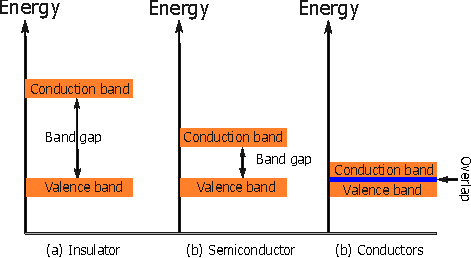
\includegraphics[width=0.8\textwidth]{fig/lec02/band_diagram.pdf}
                \caption{Energy band diagram showing the classification of materials}
            \end{figure}
\end{frame}

%%%%%%%%%%%%%%%%%%%%%%%%%%%%%%%%%%%%%%%%%%%%%%%%%%%%%%%%%%%%%
%% Energy Band diagram and classification  %%
%%%%%%%%%%%%%%%%%%%%%%%%%%%%%%%%%%%%%%%%%%%%%%%%%%%%%%%%%%%%%
\begin{frame}
	\frametitle{Energy band diagram and classification of materials}
    \begin{columns}
        \begin{column}{0.6\textwidth}
            \begin{itemize}
                \item Energy band diagram shows the energy levels of electrons in a solid material.
                \item The energy bands are separated by band gaps, which determine the electrical properties of the material.
                \item Materials can be classified based on their energy band structure:
                \begin{itemize}
                    \item Conductors: No band gap, electrons can move freely.
                    \item Semiconductors: Small band gap, electrons can be excited to the conduction band with some energy input.
                    \item Insulators: Large band gap, electrons cannot move freely without significant energy input.
                \end{itemize}
            \end{itemize}
    \end{column}
        \hfill
        \begin{column}{0.4\textwidth}
            \begin{figure}
                \centering
                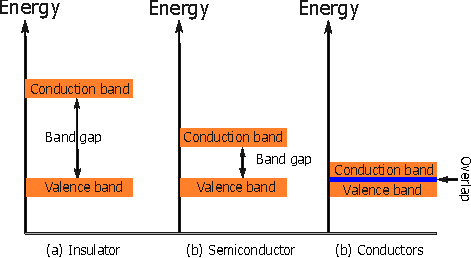
\includegraphics[width=0.8\textwidth]{fig/lec02/band_diagram.pdf}
                \caption{Energy band diagram showing the classification of materials}
            \end{figure}
        \end{column}
\end{columns}
\end{frame}

%%%%%%%%%%%%%%%%%%%%%%%%%%%%%%%%%%%%%%%%%%%%%%%%%%%%%%%%%%%%%
%% Conclusion on types of materials  %%
%%%%%%%%%%%%%%%%%%%%%%%%%%%%%%%%%%%%%%%%%%%%%%%%%%%%%%%%%%%%%
\begin{frame}
	\frametitle{Conclusion on types of materials}
    \begin{itemize}
    \item We learnt in two ways about classification of materials:
        \begin{itemize}
            \item Based on the number of valence electrons.
            \item Based on the energy band structure.
        \end{itemize}
    \end{itemize}
    \begin{columns}
        \begin{column}{0.6\textwidth}
            \begin{figure}
                \centering
                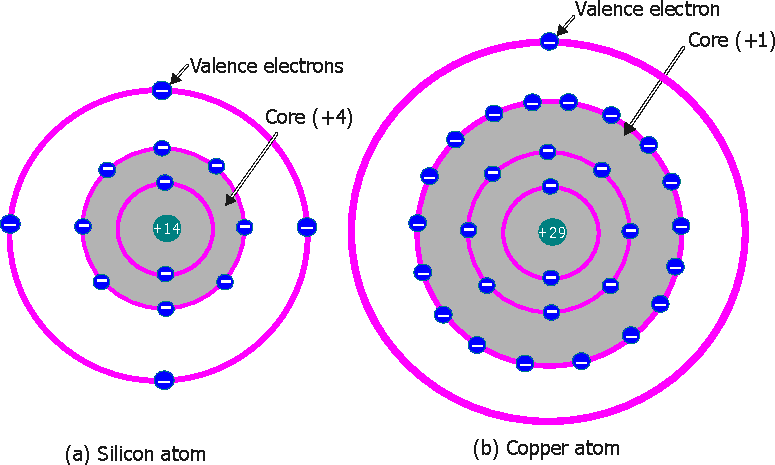
\includegraphics[width=0.6\textwidth]{fig/lec02/Cu_Si_atom1.pdf}
                \caption{(a) Silicon atom with four valence electrons, (b) Copper atom with one valence electron}
            \end{figure}
        \end{column}
        \hfill
        \begin{column}{0.4\textwidth}
            \begin{figure}
                \centering
                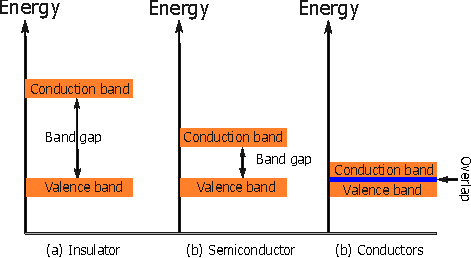
\includegraphics[width=0.6\textwidth]{fig/lec02/band_diagram.pdf}
                \caption{Energy band diagram showing the classification of materials}
            \end{figure}
        \end{column}
\end{columns}
\textbf{What next? $\rightarrow$ We will learn about the flow of electrons and holes in semiconductors.}
\end{frame}

%%%%%%%%%%%%%%%%%%%%%%%%%%%%%%%%%%%%%%%%%%%%%%%%%%%%%%%%%%%%%
%% Flow of current in semiconductors  %%
%%%%%%%%%%%%%%%%%%%%%%%%%%%%%%%%%%%%%%%%%%%%%%%%%%%%%%%%%%%%%
\begin{frame}
	\frametitle{Free electrons and holes in semiconductors}
            \begin{itemize}
                \item In semiconductors, the energy band gap is small enough that some electrons can be thermally excited from the valence band to the conduction band at room temperature.
                \item This process creates \textbf{free electrons} (also called \textbf{conduction electrons}) in the conduction band and \textbf{holes} (a vacant state that behaves like a positive charge) in the valence band.
                \item  Example: At room temperature, intrinsic silicon has enough thermal energy to excite some valence electrons across the band gap.
                \item This process results in \textbf{electron-hole pairs}.
                \item Free electrons and holes drift under electric fields and contribute to electrical conductivity.
                \item The concentration of free electrons and holes in a semiconductor can be controlled by doping with impurities.
            \end{itemize}
\end{frame}

%%%%%%%%%%%%%%%%%%%%%%%%%%%%%%%%%%%%%%%%%%%%%%%%%%%%%%%%%%%%%
%% Flow of electron current in semiconductors  %%
%%%%%%%%%%%%%%%%%%%%%%%%%%%%%%%%%%%%%%%%%%%%%%%%%%%%%%%%%%%%%
\begin{frame}
	\frametitle{Electron curent in semiconductors}
    \begin{figure}
        \centering
        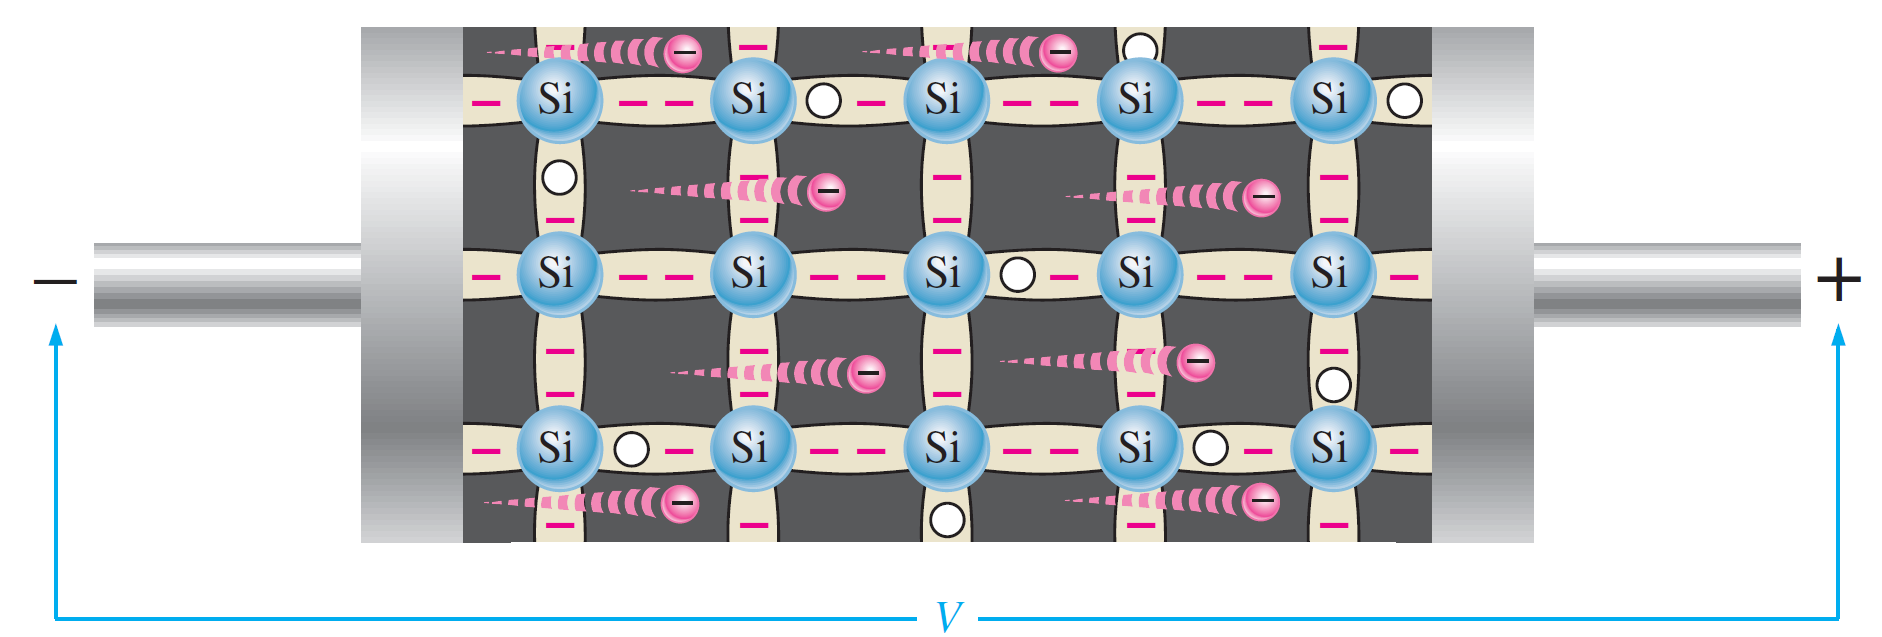
\includegraphics[width=0.75\textwidth]{fig/lec02/electron_current.png}
        \caption{Electron current in semiconductors (intrinsic Si) (Adapted from \href{https://www.pearson.com/en-us/subject-catalog/p/electronic-devices-electron-flow-version/P200000001048/9780137556755}{Electronic Devices (Electron Flow Version), 10th edition})}
    \end{figure}
    \textbf{The current we speak in general is the flow of electrons in a conductor. In semiconductors, the current is due to the flow of both electrons and holes.}
\end{frame}

%%%%%%%%%%%%%%%%%%%%%%%%%%%%%%%%%%%%%%%%%%%%%%%%%%%%%%%%%%%%%
%% Flow of hole current in semiconductors  %%
%%%%%%%%%%%%%%%%%%%%%%%%%%%%%%%%%%%%%%%%%%%%%%%%%%%%%%%%%%%%%
\begin{frame}
	\frametitle{Electron curent in semiconductors}
    \begin{figure}
        \centering
        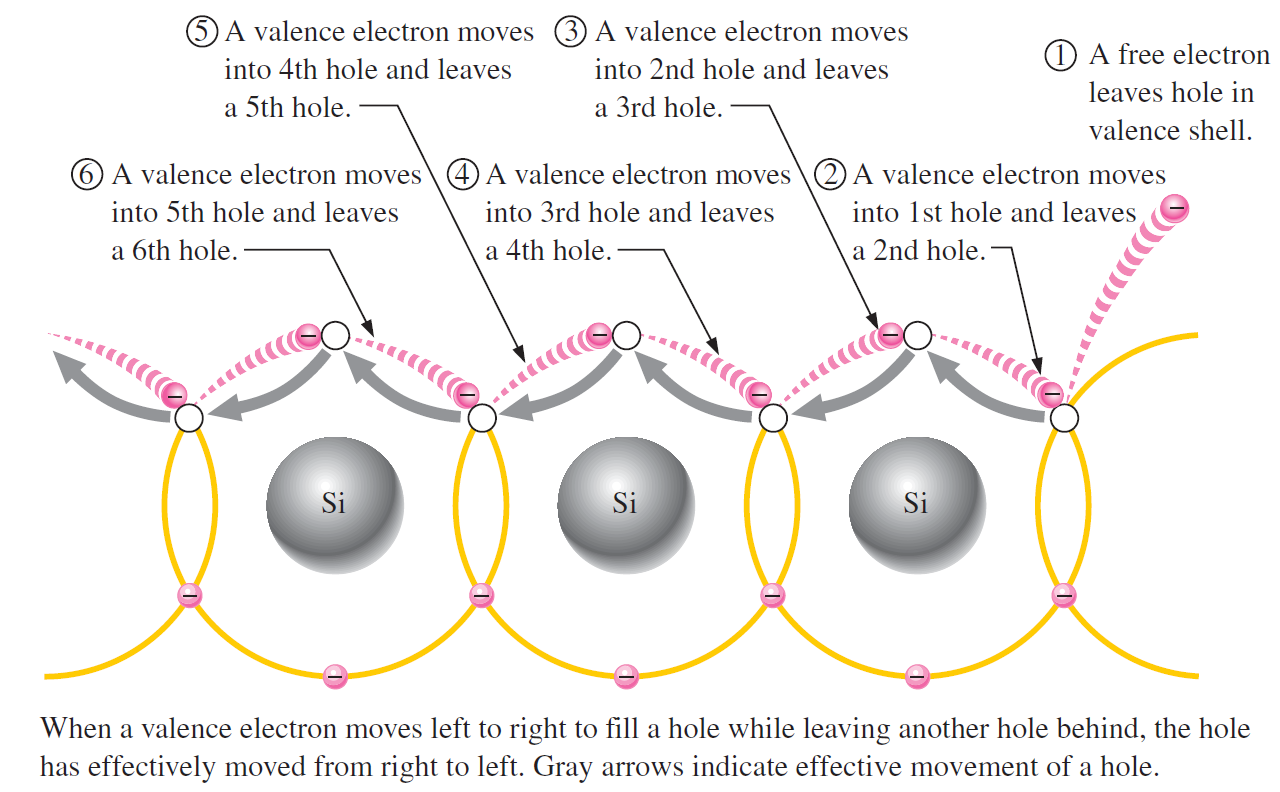
\includegraphics[width=0.65\textwidth]{fig/lec02/hole_current.png}
        \caption{Hole current in semiconductors (intrinsic Si) (Adapted from \href{https://www.pearson.com/en-us/subject-catalog/p/electronic-devices-electron-flow-version/P200000001048/9780137556755}{Electronic Devices (Electron Flow Version), 10th edition})}
    \end{figure}
\end{frame}

%%%%%%%%%%%%%%%%%%%%%%%%%%%%%%%%%%%%%%%%%%%%%%%%%%%%%%%%%%%%%
%% N-type and p-type semiconductor  %%
%%%%%%%%%%%%%%%%%%%%%%%%%%%%%%%%%%%%%%%%%%%%%%%%%%%%%%%%%%%%%
\begin{frame}
	\frametitle{N-type and P-type semiconductors}
    \begin{itemize}
        \item \textbf{Doping}: The process of adding impurities to a intrinsic (pure) semiconductor to change its electrical properties.
        \item N-type semiconductors are formed by doping intrinsic semiconductors with elements that have more valence electrons (e.g., phosphorus (P), arsenic (As)).
        \item In N-type semiconductors, the majority carriers are free electrons, while in P-type semiconductors, the majority carriers are holes.
        \item P-type semiconductors are formed by doping intrinsic semiconductors with elements that have fewer valence electrons (e.g., boron (B), gallium (Ga)).
        \item The minority carriers in N-type semiconductors are holes, while in P-type semiconductors, the minority carriers are free electrons.
    \end{itemize}
\end{frame}

%%%%%%%%%%%%%%%%%%%%%%%%%%%%%%%%%%%%%%%%%%%%%%%%%%%%%%%%%%%%%
%% Fundamental properties and terminologies  %%
%%%%%%%%%%%%%%%%%%%%%%%%%%%%%%%%%%%%%%%%%%%%%%%%%%%%%%%%%%%%%
\begin{frame}
	\frametitle{Understanding the doping process- \textbf{Donor} and Acceptor atoms}
    \begin{columns}
        \begin{column}{0.65\textwidth}
    \begin{itemize}
        \item \textbf{Donor atoms}: Atoms that donate extra electrons to the semiconductor lattice, creating N-type semiconductors.
        \item \textbf{Example of donor:} 
        \begin{itemize}
            \item Consider Germanium (Ge) as the intrinsic semiconductor. It is a group IV element with 4 valence electrons.
            \item When doped with Phosphorus (P), a group V element with 5 valence electrons, the extra electron from P becomes a free electron in the conduction band of Ge.
            \item This creates an N-type semiconductor with a higher concentration of free electrons than holes.
            \item The enrgy required to detach the extra electron from the donor atom is very small, so it is easily ionised at room temperature. For example, the ionisation energy of P in Ge is about 0.01 eV and for Si is about 0.045 eV.
        \end{itemize}    
    \end{itemize}
        \end{column}
        \hfill
        \begin{column}{0.35\textwidth}
            \begin{figure}
                \centering
                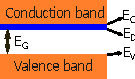
\includegraphics[scale=1.5]{fig/lec02/donor.pdf}
                \caption{Energy band diagram of an n-type semiconductor- allowable energy levels introduced in the conduction band. $E_D$ is also called Fermi level ($E_F$).}
            \end{figure}
    \end{column}
        \end{columns}
\end{frame}

%%%%%%%%%%%%%%%%%%%%%%%%%%%%%%%%%%%%%%%%%%%%%%%%%%%%%%%%%%%%%
%% Fundamental properties and terminologies  %%
%%%%%%%%%%%%%%%%%%%%%%%%%%%%%%%%%%%%%%%%%%%%%%%%%%%%%%%%%%%%%
\begin{frame}
	\frametitle{Understanding the doping process- Donor and \textbf{Acceptor atoms}}
    \begin{columns}
        \begin{column}{0.65\textwidth}
    \begin{itemize}
        \item \textbf{Acceptor atoms}: Atoms that accept electrons from the semiconductor lattice, creating P-type semiconductors.
        \item \textbf{Example of Acceptor:} 
        \begin{itemize}
            \item Consider Silicon (Si) as the intrinsic semiconductor. It is a group IV element with 4 valence electrons.
            \item When doped with Boron (B), a group III element with 3 valence electrons, the missing electron from B creates a hole in the valence band of Si.
            \item This creates a P-type semiconductor with a higher concentration of holes than free electrons.
            \item The energy required to fill the hole is very small, so it is easily ionised at room temperature. For example, the ionisation energy of B in Si is about 0.045 eV and for Ga is about 0.1 eV.
        \end{itemize}
    \end{itemize}
    \end{column}
    \hfill
    \begin{column}{0.35\textwidth}
        \begin{figure}
            \centering
            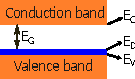
\includegraphics[scale=1.5]{fig/lec02/acceptor.pdf}
            \caption{Energy band diagram of an p-type semiconductor- allowable energy levels introduced in the valence band.  $E_D$ is also called Fermi level ($E_F$)}
        \end{figure}
    \end{column}
    \end{columns}
\end{frame}
%%%%%%%%%%%%%%%%%%%%%%%%%%%%%%%%%%%%%%%%%%%%%%%%%%%%%%%%%%%%%
%% The pn junction in a semiconductor  %%
%%%%%%%%%%%%%%%%%%%%%%%%%%%%%%%%%%%%%%%%%%%%%%%%%%%%%%%%%%%%%
\begin{frame}
	\frametitle{Acceptor and donor atoms in a semiconductor- example}
    \begin{columns}
        \begin{column}{0.5\textwidth}
            \begin{figure}
                \centering
                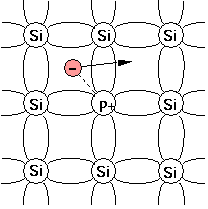
\includegraphics[scale=0.5]{fig/lec02/Donor_in_Si_lattice.png}
                \caption{Phosphorus atom acting as a donor in the simplified 2D silicon lattice. (Source: from \href{https://commons.wikimedia.org/wiki/File:Donor_in_Si_lattice.png}{Karolkalna at the English Wikipedia}, \href{http://creativecommons.org/licenses/by-sa/3.0/}{CC BY-SA 3.0})}
            \end{figure}
    \end{column}
    \hfill
    \begin{column}{0.5\textwidth}
        \begin{figure}
            \centering
            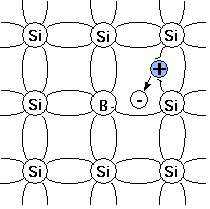
\includegraphics[scale=0.5]{fig/lec02/Acceptor_in_Si_lattice.png}
            \caption{Boron atom acting as an acceptor in the simplified 2D silicon lattice- (Source: from \href{https://commons.wikimedia.org/wiki/File:Acceptor_in_Si_lattice.png}{Karolkalna at the English Wikipedia}, \href{http://creativecommons.org/licenses/by-sa/3.0/}{CC BY-SA 3.0})}
        \end{figure}
    \end{column}
    \end{columns}
\end{frame}

%%%%%%%%%%%%%%%%%%%%%%%%%%%%%%%%%%%%%%%%%%%%%%%%%%%%%%%%%%%%%
%% Mass action law%%
%%%%%%%%%%%%%%%%%%%%%%%%%%%%%%%%%%%%%%%%%%%%%%%%%%%%%%%%%%%%%
\begin{frame}
    \frametitle{Mass action law}
    \begin{itemize}
        \item The mass action law states that the product of the concentrations of electrons and holes in a semiconductor is constant at a given temperature.
        \item This relationship can be expressed mathematically as:
        \begin{equation}
            n \cdot p = n_i^2
        \end{equation}
        where $n$ is the concentration of free electrons, $p$ is the concentration of holes, and $n_i$ is the intrinsic carrier concentration.
        \item The intrinsic carrier concentration ($n_i$) is a measure of the number of electron-hole pairs generated in an intrinsic semiconductor at thermal equilibrium.
    \end{itemize}
\end{frame}

%%%%%%%%%%%%%%%%%%%%%%%%%%%%%%%%%%%%%%%%%%%%%%%%%%%%%%%%%%%%%
% Charge Neutrality and n-Type Case
%%%%%%%%%%%%%%%%%%%%%%%%%%%%%%%%%%%%%%%%%%%%%%%%%%%%%%%%%%%%%
\begin{frame}{Charge Neutrality in Semiconductors}
    \begin{itemize}
        \item Electrical neutrality:
        \begin{equation}
        N_D + p = N_A + n 
        \end{equation}
        \item For \textbf{n-type material} ($N_A = 0$):
        \begin{equation}
        n \approx N_D 
        \end{equation}
        \item Thus, free-electron concentration equals donor atom concentration.
        \item More clearly written with subscripts:
        \begin{equation} \label{eq:charge_neutrality_n}
        n_n \approx N_D 
        \end{equation}
        \item Hole concentration:
        \begin{equation} \label{eq:charge_neutrality_p}
        p_n = \frac{n_i^2}{N_D} 
        \end{equation}
    \end{itemize}
\end{frame}
%%%%%%%%%%%%%%%%%%%%%%%%%%%%%%%%%%%%%%%%%%%%%%%%%%%%%%%%%%%%%
% p-Type Case and Doping Balance
%%%%%%%%%%%%%%%%%%%%%%%%%%%%%%%%%%%%%%%%%%%%%%%%%%%%%%%%%%%%%
\begin{frame}{p-Type Semiconductors and Doping}
    \begin{itemize}
        \item For \textbf{p-type semiconductors}:
        \begin{equation}
        p_p \approx N_A, \quad n_p = \frac{n_i^2}{N_A}
        \end{equation}
        \item Equal donor and acceptor concentrations ($N_D = N_A$) $\Rightarrow$ intrinsic behavior.
        \item Doping can switch material type depending on relative $N_D$ and $N_A$.
        \item For $N_D > N_A$, p-type becomes n-type.
        \item Adjusted neutrality (general case):
        \begin{equation}
        N_D + p = N_A + n \Rightarrow N_D - N_A = n - p
        \end{equation}
        %\item Modify Eqs. (\ref{eq:charge_neutrality_n}) and (\ref{eq:charge_neutrality_p}): Replace $N_D$ with $N_D - N_A$
    \end{itemize}
\end{frame}
%%%%%%%%%%%%%%%%%%%%%%%%%%%%%%%%%%%%%%%%%%%%%%%%%%%%%%%%%%%%%
% Conductivity in Semiconductors
%%%%%%%%%%%%%%%%%%%%%%%%%%%%%%%%%%%%%%%%%%%%%%%%%%%%%%%%%%%%%
\begin{frame}{Conductivity and Carrier Mobility}
    \begin{itemize}
        \item Semiconductors are \textbf{bipolar}: conduction via both electrons and holes.
        \item Current density:
        \begin{equation}
        J = (n \mu_n + p \mu_p)q\mathcal{E} = \sigma \mathcal{E} \tag{2-16}
        \end{equation}
        \item $n$, $p$: carrier concentrations; $\mu_n$, $\mu_p$: mobilities.
        \item Conductivity:
        \begin{equation}
        \sigma = (n \mu_n + p \mu_p)q \tag{2-17}
        \end{equation}
        \item Intrinsic case: $n = p = n_i$
    \end{itemize}
\end{frame}

%%%%%%%%%%%%%%%%%%%%%%%%%%%%%%%%%%%%%%%%%%%%%%%%%%%%%%%%%%%%%
% Temperature Dependence of Intrinsic Carriers
%%%%%%%%%%%%%%%%%%%%%%%%%%%%%%%%%%%%%%%%%%%%%%%%%%%%%%%%%%%%%
\begin{frame}{Intrinsic Carrier Concentration and Temperature Dependence}
    \begin{itemize}
        \item As temperature increases, intrinsic carrier concentration increases:
        \begin{equation}
        n_i^2 = A_0 T^3 e^{-E_{G0}/kT} \tag{2-18}
        \end{equation}
        \item Temperature-dependent bandgap:
        \begin{equation}
        E_G(T) = 1.21 - 3.60 \times 10^{-4}T \quad \text{(Si)} \tag{2-19}
        \end{equation}
        \begin{equation}
        E_G(T) = 0.785 - 2.23 \times 10^{-4}T \quad \text{(Ge)} \tag{2-20}
        \end{equation}
        \item As $T$ increases:
        \begin{itemize}
            \item $E_G$ decreases
            \item $n_i$ increases
            \item Conductivity increases
        \end{itemize}
    \end{itemize}
\end{frame}


%%%%%%%%%%%%%%%%%%%%%%%%%%%%%%%%%%%%%%%%%%%%%%%%%%%%%%%%%%%%%
% The Hall Effect - Introduction
%%%%%%%%%%%%%%%%%%%%%%%%%%%%%%%%%%%%%%%%%%%%%%%%%%%%%%%%%%%%%
\begin{frame}{The Hall Effect}
\begin{columns}
    \begin{column}{0.5\textwidth}
    \begin{itemize}
        \item When a semiconductor carries a current $I$ in a transverse magnetic field $B$, an electric field $\mathcal{E}$ develops perpendicular to both $I$ and $B$.
        \item This phenomenon is known as the \textbf{Hall Effect}.
        \item Used to determine:
        \begin{itemize}
            \item Whether a semiconductor is \textbf{n-type} or \textbf{p-type}
            \item The carrier concentration
            \item The mobility $\mu$ of carriers
        \end{itemize}
        \item A potential difference, called the \textbf{Hall voltage} $V_H$, appears across the sample.
    \end{itemize}
\end{column}
\begin{column}{0.5\textwidth}
    \begin{figure}[h]
        \centering
        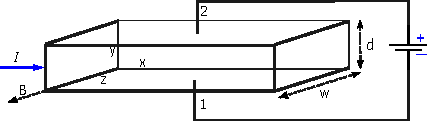
\includegraphics[width=1\textwidth]{fig/lec02/hall_effect.pdf} % Replace with your actual image file
        \caption{Schematic diagram of Hall setup showing force on charge carriers}
    \end{figure}
\end{column}
\end{columns}
\end{frame}

%%%%%%%%%%%%%%%%%%%%%%%%%%%%%%%%%%%%%%%%%%%%%%%%%%%%%%%%%%%%%
% Hall Effect - Physical Explanation
%%%%%%%%%%%%%%%%%%%%%%%%%%%%%%%%%%%%%%%%%%%%%%%%%%%%%%%%%%%%%
\begin{frame}{Lorentz Force and Hall Field}
    \begin{itemize}
        \item Consider a semiconductor sample placed in a magnetic field $\vec{B}$ in the $z$-direction.
        \item A current $I$ is passed in the $x$-direction, perpendicular to $\vec{B}$.
        \item Charge carriers (electrons or holes) moving with velocity $\vec{v}$ experience a force:
        \begin{equation}
        \vec{F} = q(\vec{v} \times \vec{B})
        \end{equation}
        \item This Lorentz force deflects carriers in the $+y$ direction, creating:
        \begin{itemize}
            \item Negative charge on the $+y$ side (if electrons dominate)
            \item Positive charge on the $-y$ side
        \end{itemize}
        \item This generates an electric field $E_H$ opposing the Lorentz force:
        \begin{equation} \label{eq:Lorentz_force}
        \vec{F} = q(\vec{E} + \vec{v} \times \vec{B}) = 0 
        \end{equation}
        For simplicity, let's represent $\vec{E}=\mathcal{E}$
    \end{itemize}
\end{frame}

%%%%%%%%%%%%%%%%%%%%%%%%%%%%%%%%%%%%%%%%%%%%%%%%%%%%%%%%%%%%%
% Hall Field and Charge Type Identification
%%%%%%%%%%%%%%%%%%%%%%%%%%%%%%%%%%%%%%%%%%%%%%%%%%%%%%%%%%%%%
\begin{frame}{Hall Voltage and Carrier Type}
    \begin{itemize}
        \item Solving Eq. \ref{eq:Lorentz_force} gives the Hall field:
        \begin{equation}
            \mathcal{E} = v_x B_z 
        \end{equation}
        \item This field gives rise to a Hall voltage:
        \begin{equation}
        V_H = d \mathcal{E} = d v_x B_z
        \end{equation}
        \item $d$: width of the semiconductor sample
        \item Since current $I \propto q v_x$, the sign of $V_H$ indicates:
        \begin{itemize}
            \item $V_H > 0$: Majority carriers are electrons (n-type)
            \item $V_H < 0$: Majority carriers are holes (p-type)
        \end{itemize}
        \item Thus, \textbf{Hall effect enables determination of carrier type} in semiconductors
    \end{itemize}
\end{frame}

%%%%%%%%%%%%%%%%%%%%%%%%%%%%%%%%%%%%%%%%%%%%%%%%%%%%%%%%%%%%%
% Derivation of Hall Voltage
%%%%%%%%%%%%%%%%%%%%%%%%%%%%%%%%%%%%%%%%%%%%%%%%%%%%%%%%%%%%%

\begin{frame}{Experimental Determination of $\mu$ (mobility of charge carrier) and $\rho$ (charge density)}
    \begin{itemize}
        \item In the equilibrium state the electric field intensity $\mathcal{E}$ due to Hall effect must be equal to the magnetic force:
        \begin{equation}
        q\mathcal{E} = Bqv \tag{2-21}
        \end{equation}
        \item Using $\mathcal{E} = \frac{V_H}{d}$ and $J = \rho v = \frac{I}{wd}$, where $\rho$ is the charge density, $w$ is the width of the sample, and $J$ is the current density:
        \begin{equation}
        V_H = \mathcal{E}d = Bvd = \frac{BJd}{\rho} = \frac{BI}{\rho w} \tag{2-22}
        \end{equation}
        \item Hence $\rho$ can be expressed as:
        \begin{equation}
        \rho = \frac{BI}{V_H w} \Rightarrow R_H = \frac{1}{\rho} = \frac{V_H w}{BI} \tag{2-23, 2-24}
        \end{equation}
        where $R_H$ is the Hall coefficient.
    \end{itemize}
\end{frame}

%%%%%%%%%%%%%%%%%%%%%%%%%%%%%%%%%%%%%%%%%%%%%%%%%%%%%%%%%%%%%
% Mobility from Hall Coefficient
%%%%%%%%%%%%%%%%%%%%%%%%%%%%%%%%%%%%%%%%%%%%%%%%%%%%%%%%%%%%%
\begin{frame}{Hall Coefficient and Mobility}
    \begin{itemize}
        \item Conductivity: $\sigma = \rho \mu$ (for single carrier type)
        \item Therefore, mobility:
        \begin{equation}
        \mu = \sigma R_H \tag{2-26}
        \end{equation}
        \item If random thermal motion is accounted for:
        \begin{equation}
        \mu = \left( \frac{8\sigma}{3\pi} \right) R_H
        \end{equation}
        \item Hall effect allows complete characterization of a semiconductor.
    \end{itemize}
\end{frame}

%%%%%%%%%%%%%%%%%%%%%%%%%%%%%%%%%%%%%%%%%%%%%%%%%%%%%%%%%%%%%
% Applications and Conductivity Modulation
%%%%%%%%%%%%%%%%%%%%%%%%%%%%%%%%%%%%%%%%%%%%%%%%%%%%%%%%%%%%%
\begin{frame}{Applications and Conductivity Modulation}
    \begin{itemize}
        \item Applications:
        \begin{itemize}
            \item Magnetic field sensors (Hall-effect meters)
            \item Hall-effect multipliers (measure product of two signals)
        \end{itemize}
        \item Conductivity $\sigma$ can be modulated by:
        \begin{itemize}
            \item Varying temperature
            \item Doping to increase $n$ or $p$
            \item Illumination to generate electron-hole pairs
        \end{itemize}
        \item Reiterates Eq. (2-17): $\sigma = (n\mu_n + p\mu_p)q$
    \end{itemize}
\end{frame}

%%%%%%%%%%%%%%%%%%%%%%%%%%%%%%%%%%%%%%%%%%%%%%%%%%%%%%%%%%%%%
% Carrier Generation and Recombination
%%%%%%%%%%%%%%%%%%%%%%%%%%%%%%%%%%%%%%%%%%%%%%%%%%%%%%%%%%%%%

\begin{frame}{Carrier Generation and Recombination}

    \begin{itemize}
        \item \textbf{Generation}: Creation of electron-hole pairs (EHPs)
        \begin{itemize}
            \item Due to thermal energy or light (photons)
        \end{itemize}
        \item \textbf{Recombination}: Annihilation of an electron with a hole
        \item At equilibrium, generation rate $G$ equals recombination rate $R$
        \item Important for determining carrier lifetime $\tau$: Average time a carrier exists before recombination.
        \item \textbf{Auger recombination}: Involves three carriers (two electrons and one hole or vice versa). 
        \begin{itemize}
            \item It it transfer of the energy and momentum released by the recombination of an electron-hole pair to a third mobile particle- electrons in the case of heavily doped N-type material and holes in the case of heavily doped P-type material.
            \item It is a non-radiative process and is the dominant recombination mechanism in heavily doped semiconductors.
            \item Auger recombination is a significant factor in determining the efficiency of semiconductor devices, especially in \textbf{high-power and high-frequency applications}.
        \end{itemize}
        \item \textbf{Radiative recombination}: Involves emission of a photon.
    \end{itemize}

\end{frame}

%%%%%%%%%%%%%%%%%%%%%%%%%%%%%%%%%%%%%%%%%%%%%%%%%%%%%%%%%%%%%
% Carrier Diffusion
%%%%%%%%%%%%%%%%%%%%%%%%%%%%%%%%%%%%%%%%%%%%%%%%%%%%%%%%%%%%%

\begin{frame}{Carrier Diffusion}
    \begin{itemize}
        \item Caused by spatial concentration gradients of charge carriers
        \item Electrons and holes move from regions of high to low concentration
        \item Electron diffusion current density:
        \begin{equation}
        J_n^{\text{diff}} = q D_n \frac{dn}{dx}
        \end{equation}
        \item Hole diffusion current density:
        \begin{equation}
        J_p^{\text{diff}} = -q D_p \frac{dp}{dx}
        \end{equation}
        \item Where:
        \begin{itemize}
            \item $q$: elementary charge
            \item $D_n$, $D_p$: diffusion coefficients of electrons and holes
            \item $\frac{dn}{dx}$, $\frac{dp}{dx}$: gradients of electron and hole concentrations with respect to position $x$
        \end{itemize}
    \end{itemize}
\end{frame}

%%%%%%%%%%%%%%%%%%%%%%%%%%%%%%%%%%%%%%%%%%%%%%%%%%%%%%%%%%%%%
% Carrier Drift
%%%%%%%%%%%%%%%%%%%%%%%%%%%%%%%%%%%%%%%%%%%%%%%%%%%%%%%%%%%%%
\begin{frame}{Carrier Drift}
    \begin{itemize}
        \item Caused by an applied electric field $\mathcal{E}$ across the semiconductor
        \item Electron drift current:
        \begin{equation}
        J_n^{\text{drift}} = q n \mu_n \mathcal{E}
        \end{equation}
        \item Hole drift current:
        \begin{equation}
        J_p^{\text{drift}} = q p \mu_p \mathcal{E}
        \end{equation}
        \item Where:
        \begin{itemize}
            \item $n$, $p$: concentrations of electrons and holes
            \item $\mu_n$, $\mu_p$: mobilities of electrons and holes
            \item $\mathcal{E}$: electric field (V/m)
        \end{itemize}
        \item Drift current is proportional to the electric field and carrier concentration
        \item Drift and diffusion currents are the two main mechanisms of charge transport in semiconductors
    \end{itemize}
\end{frame}



%%%%%%%%%%%%%%%%%%%%%%%%%%%%%%%%%%%%%%%%%%%%%%%%%%%%%%%%%%%%%
% Drift vs Diffusion
%%%%%%%%%%%%%%%%%%%%%%%%%%%%%%%%%%%%%%%%%%%%%%%%%%%%%%%%%%%%%
\begin{frame}{Distinction: Drift vs Diffusion Currents}
    \centering
    \textbf{Comparison of Drift and Diffusion Currents} \\[1ex]
    \begin{tabular}{|p{3cm}|p{4cm}|p{4cm}|}
        \hline
        \textbf{Aspect} & \textbf{Drift Current} & \textbf{Diffusion Current} \\
        \hline
        Driving Force & Electric field ($\mathcal{E}$) & Concentration gradient ($\frac{dn}{dx}$ or $\frac{dp}{dx}$) \\
        \hline
        Direction & Field direction & High to low concentration \\
        \hline
        Equation & $q n \mu \mathcal{E}$ or $q p \mu \mathcal{E}$ & $q D \frac{dn}{dx}$ or $-q D \frac{dp}{dx}$ \\
        \hline
        Occurs Due To & External bias & Inhomogeneous doping or illumination \\
        \hline
        Field Requirement & Required & Not required \\
        \hline
    \end{tabular}
\end{frame}

%%%%%%%%%%%%%%%%%%%%%%%%%%%%%%%%%%%%%%%%%%%%%%%%%%%%%%%%%%%%%
% RElating mobility and diffusion of charge carriers
%%%%%%%%%%%%%%%%%%%%%%%%%%%%%%%%%%%%%%%%%%%%%%%%%%%%%%%%%%%%%
\begin{frame}{How mobility and diffusion are related of charge carrier are related?}
    \begin{itemize}
        \item \textbf{Mobility} ($\mu$): Measure of how quickly charge carriers (electrons or holes) can move through a semiconductor material in response to an electric field.
        \item \textbf{Diffusion coefficient} ($D$): Measure of how quickly charge carriers can spread out in a semiconductor material due to concentration gradients.
        \item \textbf{Einstein relation}: Connects mobility and diffusion coefficient:
        \begin{equation}
        D = \frac{kT}{q} \mu    
        \end{equation}
        \item Where:
        \begin{itemize}
            \item $k$: Boltzmann constant
            \item $T$: Absolute temperature (in Kelvin)
            \item $q$: Elementary charge (charge of an electron)
        \end{itemize}
        \item This relation shows that the diffusion coefficient is directly proportional to the mobility of charge carriers and the temperature.
        \item Higher mobility leads to higher diffusion rates, which is important for understanding charge transport in semiconductors.
    \end{itemize}
    \end{frame}

    %%%%%%%%%%%%%%%%%%%%%%%%%%%%%%%%%%%%%%%%%%%%%%%%%%%%%%%%%%%%%
% RElating mobility and diffusion of charge carriers
%%%%%%%%%%%%%%%%%%%%%%%%%%%%%%%%%%%%%%%%%%%%%%%%%%%%%%%%%%%%%
\begin{frame}{Relevance of Einstein relation?}
    \begin{itemize}
        \item The Einstein relation is a fundamental concept that bridge the microscopic thermal motion of carriers with their macroscopic electrical behavior, and is essential for modeling how semiconductors behave under various conditions.
        \item \textbf{Unifies Drift and Diffusion:} Shows that mobility (drift due to electric field) and diffusion (due to concentration gradient) are inherently linked by thermal motion.
        \item \textbf{Device Modeling:} Essential for modeling carrier transport in semiconductors such as diodes, BJTs, and MOSFETs where both drift and diffusion processes coexist.
        \item \textbf{Simplifies Analysis:} If one parameter (e.g., mobility) is known, diffusion coefficient can be calculated, reducing experimental complexity.
        \item \textbf{Temperature Dependence:} Since $D \propto T$ and $\mu \propto T^{-m}$ (where $m \approx 1.5$), the Einstein relation captures how transport properties change with temperature — crucial for thermal sensor and reliability design.
        \item \textbf{Measurement and Material Characterization:} Enables calculation of diffusion coefficient $D$ from mobility $\mu$ measured using Hall effect.
    \end{itemize}
\end{frame}

%%%%%%%%%%%%%%%%%%%%%%%%%%%%%%%%%%%%%%%%%%%%%%%%%%%%%%%%%%%%%
% Deriving the Einstein Relation
%%%%%%%%%%%%%%%%%%%%%%%%%%%%%%%%%%%%%%%%%%%%%%%%%%%%%%%%%%%%%
\begin{frame}{Deriving Einstein Relation}
    \begin{itemize}
        \item The Einstein relation connects the diffusion coefficient ($D$) and the mobility ($\mu$) of charge carriers in thermal equilibrium.
        \item For electrons:
        \begin{equation}
        D_n = \frac{kT}{q} \mu_n, \quad \text{and for holes: } D_p = \frac{kT}{q} \mu_p
        \end{equation}
        \item \textbf{Start with the drift current:} 
        \begin{equation}
        J_n^{\text{drift}} = q n \mu_n \mathcal{E}
        \end{equation}
        \item \textbf{In equilibrium}, the total electron current must be zero:
        \begin{equation}
        J_n^{\text{drift}} + J_n^{\text{diff}} = 0
        \Rightarrow q n \mu_n \mathcal{E} + q D_n \frac{dn}{dx} = 0
        \end{equation}
    \end{itemize}
\end{frame}

\begin{frame}{Deriving Einstein Relation. Contd.}
    \begin{itemize}
        \item From Boltzmann distribution:
        \begin{equation}
        n(x) \propto e^{-q\phi(x)/kT} \Rightarrow \frac{dn}{dx} = \frac{q n \mathcal{E}}{kT}
        \end{equation}
        \item Substituting back into current balance:
        \begin{align*}
        q n \mu_n \mathcal{E} + q D_n \left( \frac{q n \mathcal{E}}{kT} \right) &= 0 \\
        \Rightarrow q n \mathcal{E} \left( \mu_n + \frac{q D_n}{kT} \right) &= 0
        \end{align*}
        \item Since $q n \mathcal{E} \neq 0$ in general, we get:
        \begin{equation}
        D_n = \frac{kT}{q} \mu_n
        \end{equation}
        \item Similarly, for holes:
        \begin{equation}
        D_p = \frac{kT}{q} \mu_p
        \end{equation}
    \end{itemize}
\end{frame}

%%%%%%%%%%%%%%%%%%%%%%%%%%%%%%%%%%%%%%%%%%%%%%%%%%%%%%%%%%%%%
% Continuity Equation
%%%%%%%%%%%%%%%%%%%%%%%%%%%%%%%%%%%%%%%%%%%%%%%%%%%%%%%%%%%%%
\begin{frame}{Continuity Equation}
    \begin{itemize}
        \item Expresses conservation of charge carriers over time and space and ensured that the total charge in a semiconductor remains constant or the law of \textbf{conservation of charge}.
        \item For electrons:
        \begin{equation}
        \frac{\partial n}{\partial t} = \frac{1}{q} \frac{\partial J_n}{\partial x} + G_n - R_n
        \end{equation}
        \item Where:
        \begin{itemize}
            \item $n$: electron concentration (per unit volume)
            \item $J_n$: electron current density
            \item $G_n$: electron generation rate
            \item $R_n$: electron recombination rate
        \end{itemize}
        \item Similar form exists for holes
        \item Important in analyzing transient or steady-state carrier dynamics
    \end{itemize}
\end{frame}

%%%%%%%%%%%%%%%%%%%%%%%%%%%%%%%%%%%%%%%%%%%%%%%%%%%%%%%%%%%%%
% Continuity Equation
%%%%%%%%%%%%%%%%%%%%%%%%%%%%%%%%%%%%%%%%%%%%%%%%%%%%%%%%%%%%%
\begin{frame}{Continuity Equation- relevance}
    \begin{itemize}
        \item Models \textbf{transient behavior} in devices (e.g., switching in transistors, photodiode response), basically how quickly a device responds to changes in input.
        \item Describes \textbf{steady-state operation} when $\partial n/\partial t = 0$, hence used in diode forward and reverse bias analysis, minority carrier injection in BJTs.
        \item Forms the backbone of \textbf{minority carrier analysis} in diodes and BJTs
        \item Extends to holes: \( \frac{\partial p}{\partial t} = -\frac{1}{q} \frac{\partial J_p}{\partial x} + G_p - R_p \), together with the electron equation, allows for a complete description of carrier dynamics in semiconductors.
        \item Couples with Poisson’s equation (describes how the electric potential varies in space due to the presence of electric charge within the material) for \textbf{complete device modeling} 
        \item Core equation in numerical tools like TCAD, COMSOL, Silvaco
    \end{itemize}
\end{frame}

%%%%%%%%%%%%%%%%%%%%%%%%%%%%%%%%%%%%%%%%%%%%%%%%%%%%%%%%%%%%%
% Impact Ionisation and Avalanche Breakdown
%%%%%%%%%%%%%%%%%%%%%%%%%%%%%%%%%%%%%%%%%%%%%%%%%%%%%%%%%%%%%
\begin{frame}{Impact Ionization}
    \begin{itemize}
        \item \textbf{Impact ionization}: Process where a high-energy electron collides with an atom, creating an electron-hole pair.
        \item This process can lead to a chain reaction, where the newly created electrons also gain enough energy to create more electron-hole pairs.
        \item Impact ionization is a high-field carrier generation mechanism leading to \textbf{avalanche multiplication}.
        \item It occurs when electrons or holes in a strong electric field gain sufficient kinetic energy to ionize atoms, creating electron-hole pairs.
        \item Fundamental in determining the \textbf{breakdown voltage} in devices like diodes and power MOSFETs.
        \item Before we proceed, just a short thought on how a device conducts current.
            \begin{itemize}
                \item In forward bias, due to diffusion of majority carriers, the depletion region shrinks and the current increases exponentially with voltage.
                \item In reverse bias, If voltage is low and doping is high $\rightarrow$ Zener breakdown, \\
                If voltage is high and doping is low $\rightarrow$ Avalanche breakdown
            \end{itemize}
    \end{itemize}
\end{frame}    